\documentclass[12pt]{report}
\usepackage[a4paper, margin=0.5in]{geometry}
\usepackage{graphicx, wrapfig, hyperref, amsmath, amssymb, geometry, array, float}
\renewcommand{\familydefault}{\sfdefault}
\usepackage[scaled]{helvet}
\usepackage[table]{xcolor}
\geometry{margin=1in}


\usepackage{titlesec}

\titleformat{\chapter}[display]
  {\normalfont\huge\bfseries}{}{0pt}{\Huge\vspace{-2cm}} % you can tweak this

\titlespacing*{\chapter}{0pt}{5pt}{20pt} % left, before, after


\begin{document}

% ====================== TITLE ========================
  \begin{center}
    % \vspace*{-1in}
    
\includegraphics[width=0.4\textwidth]{sae_aerospace.png}\\
    \vspace{1cm}
    \textbf{\LARGE AEROTHON 2025} \\
    \vspace{0.5in}
    \textbf{\Large UNCREWED AIRCRAFT SYSTEM  (UAS) \\
    DESIGN, BUILD \\ AND FLY CONTEST}\\
    \vspace{0.5cm}
    
\includegraphics[width=0.4\textwidth]{aerothon2025.png}\\
    \vspace{0.5cm}
    \Large \textbf{PHASE 1:} DESIGN REPORT \\
    \vspace{0.5cm}
    \Large \textbf{TEAM NAME:} UDSAV \\
    \Large \textbf{TEAM NUMBER: } AT2025043
    
    \vspace{0.5cm}
    
\includegraphics[width=0.3\textwidth]{gsvlogo.png}\\
    \vspace{0.5cm}
    \textbf{\Large GATI SHAKTI VISHWAVIDYALAYA} \\
    \large{Ministry of Railways, Govt. of India \\Vadodara, India - 390004}
  \end{center}
  % ======================================================
  \newpage
  \begin{figure}[h] 
    \centering
    
\includegraphics[width=1\textwidth]{certificate_faculty.jpeg}
  \end{figure}
  \newpage

  \newgeometry{left=1in, right=0.5in, top=1in, bottom=0.5in}
  % ============ [TABLE OF CONTENTS] ================
  \tableofcontents
  \newpage

  \newgeometry{left=1in, right=0.5in, top=0.5in, bottom=0.5in}
  \renewcommand{\arraystretch}{1.5}
      \rowcolors{1}{white}{blue!10}

  % ================== Introduction =================
  \chapter{Introduction}
  \section{Overview}

   In the face of natural and man-made disasters, rapid response and situational awareness are critical. Drones have emerged as powerful tools in disaster management, offering real-time aerial insights, access to hard-to-reach areas, and faster deployment compared to traditional methods. Whether locating survivors, assessing damage, or delivering essential supplies, drone technology enhances the efficiency and safety of relief operations. As disasters grow more complex and unpredictable, integrating drones into emergency response systems is no longer a luxury—it's a necessity. \\ 

   Through Aerothon, Team UDSAV (\textit{Uncrewed Disaster Surveillance Aerial Vehicle}) is not just competing—we are contributing to the evolution of drone-assisted disaster response, pushing the boundaries of what UAVs can achieve in life-saving missions.

    \section{Problem Statement and Mission Requirements}
    This year's AEROTHON is themed on \textbf{\textit{Surveillance and Disaster Management.}} The problem statement is to build an \textbf{\textit{Uncrewed Aircraft System (UAS)}} to be able to perform the mission requirements as per the rulebook. The mission requirements at a glance are as follows: \\ \\
    \textbf{Mission - 1:} \textit{Advanced Obstacle Navigation $\&$ Fragile Payload Delivery with Precision Placement – Manual Operation} \\ \\
    \textbf{Mission - 2:} \textit{Autonomous Object Classification, Disaster Situation Identification $\&$ Payload Drop – Autonomous Operation} 



    \section{Scope of Report}
    The scope of this report is to provide a comprehensive understanding of the design rationale we have used while building this project. We have tried to provide the relevant calculations, figures, and analysis models to justify the materials/design/framework we've chosen to work with for our structural and system architectures. \\ 

    \noindent Apart from that, this report is intended to also serve as an accessible guide catering to neophytes in UAV/UAS systems. We have tried our best to aim at providing clear context and insight that sort of demystifies drone development. \\

  % ======== Requirements and Design Objectives =========
  \section{System Requirements \& Design Objectives}
    \subsection{Mission Profile}
    \begin{enumerate}
      \item \textbf{Mission 1:} \textit{Advanced Obstacle Navigation $\&$ Fragile Payload Delivery with Precision Placement} \\
        This is a \textbf{\textit{Manual Operation.}} In this mission, the drone must transport a fragile payload through a challenging course filled with static obstacles such as walls, barriers, and narrow passages. The primary objective is to navigate these obstacles with high precision while ensuring the payload remains undamaged. \\
        
        Upon reaching the target zone, the drone must land carefully and place the fragile payload on the ground without causing any damage. After the successful placement, the drone must then return to the takeoff point or designated home base, ensuring safe and efficient navigation back through the course. The mission is complete once the payload is placed securely, and the drone successfully returns to the home base.
      \item \textbf{Mission 2:} \textit{Autonomous Object Classification, Disaster Situation Identification $\&$ Payload Drop }\\
        This is an \textbf{\textit{Autonomous Operation.}} In this mission, the drone will autonomously scan, classify, and assess objects within a predefined area using onboard sensors and algorithms. The objects will vary in shape, size, color, and structure, and may be partially obscured, presenting challenges for detection and classification. Once the objects are classified, the drone will identify potential disaster scenarios, such as flooding, fire, or damaged infrastructure, within the same area.
    \end{enumerate}
    \subsection{Key Performance Indicators \& Constraints}
    According to the above defined mission profiles, we have a few KPIs (\textit{Key Performance Index}) to keep in mind.
    \begin{enumerate}
      \item Flight Endurance and Range 
      \item Payload Handling 
      \item Autonomous Capabilites
      \item System Reliability
      \item Design and Innovation
    \end{enumerate}
        The design and development of the UAV is subjected to several constraints as per the guidelines mentioned in the rulebook AEROTHON 2025. These include dimensional constraints, payload restrictions and strict autonomy requirements. The drone must perform all missions bound by these constraints and we have taken great time and care to articulate them down to ensure nothing is amiss.
    \begin{enumerate}
      \item \textbf{Dimensional Constraints}
        \begin{itemize}
          \item Maximum Wingspan: \textbf{1.5 metres} - the UAV must fit inside a \textbf{\textit{1.5m x 1.5m x 1.5m bounding box}} in assembled condition.
          \item Maximum Takeoff Weight: \textbf{3.5kg} including battery and payload.
        \end{itemize}
      \item \textbf{Payload Constraints}
        \begin{itemize}
          \item Payload: One fragile payload cube of \textbf{\textit{10cm x 10cm x 10cm}} weighing \textbf{\textit{150 ~ 200g}}.
          \item Payload must be released within a \textbf{\textit{3m x 3m}} target zone.
        \end{itemize}
      \item \textbf{Flight Environment Constraints}
        \begin{itemize}
          \item Missions are conducted in \textbf{\textit{open outdoor airspace}}.
          \item Expect wind speeds upto \textbf{\textit{5m/s}}
        \end{itemize}
      \item \textbf{Autonomy and Mission Constraints}
        \begin{itemize}
          \item \textbf{Mission 1:} Manual flight only (no GPS or autopilot usage).
          \item \textbf{Mission 2:} Fully autonomous flight (no pilot intervention or RC use).
          \item All autonomous missions must avoid obstacles and make decisions based on \textbf{\textit{onboard computation.}}
        \end{itemize}
      \item \textbf{Power and Communication Constraints}
        \begin{itemize}
          \item Must operate on battery only
          \item No cellular or internet-based comms allowed
          \item Only 2.4 GHz or 5.8 GHz RF modules permitted
        \end{itemize}
      \item \textbf{Safety and Compliance}
        \begin{itemize}
          \item Must have a failsafe mode (e.g., return-to-home or emergency land)
          \item Must pass technical inspection before flying
          \item Compliance with DGCA drone guidelines (if relevant in test zones)
        \end{itemize}
      \item \textbf{Operational Constraints}
        \begin{itemize}
          \item The team must complete the flight within a \textbf{\textit{15-minute slot.}}
          \item Payload must be dropped in an area of \textbf{\textit{3m x 3m.}}
        \end{itemize}
    \end{enumerate}
  % ========= Conceptual Design Approach =======
  \chapter{Conceptual Design Approach}
    \section{Design Methodology}
    \section{Product Benchmark \& Trade-off Analysis} % why we chose this design over other 
                                                 
  % ======== Aerodynamic and Flight Performance ======
  \chapter{Detailed Design Breakdown}                                 
    \section{Preliminary Weight Estimation}
      \begin{table}[H]
      \centering
      \caption{Detailed Weight Breakdown}
        \begin{tabular}{|>{\raggedright\arraybackslash}p{6cm}|>{\raggedright\arraybackslash}p{6cm}|}
          \hline
          \textbf{Parameter} & \textbf{Weight \textit{(gms)}} \\
          \hline
          NVIDIA Jetson Orin Nano & 176 \\
          Pixhawk 2.4.8	& 39 \\
          Camera (\textit{x2})	 & 20 \\
          SpeedyBee BL32 50A 4-in-1 ESC	& 90 \\
          DYS D2836-7 1120KV BLDC (\textit{x4}) &	280 \\
          Battery	& --  \\
          GPS – Neo M8N & 	23  \\
          Transmitter (SkyDroid) & 	17 \\
          Receiver & -- \\
          Payload	& 200 \\
          Additional Wiring & 50 \\
          Servo Motor & 10 \\
          Propellor (9") & -- \\
          Estimated Frame Weight & 500 \\
          \hline
          \textbf{\textit{Total:}} & -- \\
          \hline
        \end{tabular}
      \end{table}
      
  % ============== Propulsion ====================
    \section{Thrust Requirement \& Propulsion System Selection}
      \subsection{Motor, ESC \& Propellor}
      \vspace{0.5cm}
      
      \subsubsection{Motor: DYS D2836-7 1120KV Brushless Motor} 
      \begin{wrapfigure}{r}{0.2\textwidth}
        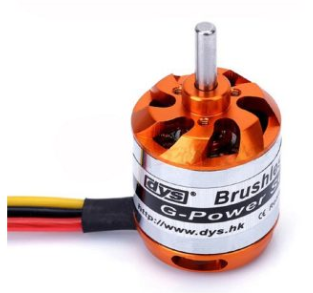
\includegraphics[width=0.2\textwidth]{bldc.png}
        \caption{DYS D2836-7 1120kV BLDC}
        \label{fig:bldc1120}
      \end{wrapfigure}
      The DYS D2836-7 1120KV Brushless Motor is our go-to motor for this project because of the following leverages it offers:
        
      \begin{itemize}
        \item \textbf{\textit{KV Rating: 1120KV}} - KV generally means RPM per volt. In layman terms, in one volt, how many rotations does it make per minute = KV. In this case, 1120KV is mid-range, which means good thrust at moderate RPMs, and it works decently with larger propellors (\textit{9" - 11"}) which improves lift and efficiency, \textit{especially} at low speeds. This is perfect for surveillance drones that require loitering and stability. A lower KV would force us to use bulky propellors, and a higher KV would drain the battery faster. 1120KV is a sweet spot between the two.
        \item \textbf{\textit{Power \& Efficiency:}} - With a 3S or 4S LiPo, this motor produces ~800g to 1100g of thrust, depending on the propeller used. It can pull 20–25A max, so it's efficient for mid-weight UAVs (\textit{in our case, it is around \textbf{1.5 ~ 2kg AUW} (All Up Weight.)}), so it's ideal for our choice.
      \end{itemize}
      
      
      \begin{table}[H]
      \centering
      \caption{Motor Datasheet (DYS D2836-7 1120kV BLDC)}
        \begin{tabular}{|>{\raggedright\arraybackslash}p{6cm}|>{\raggedright\arraybackslash}p{6cm}|}
          \hline
          \textbf{Parameter} & \textbf{Value} \\
          \hline
          Motor KV (RPM/V) & 1120 \\
          \hline
          Motor Type & Brushless Motor \\
          \hline
          Compatible LiPO Batteries & 2S to 4S \\
          \hline
          Weight (g) & 70 \\
          \hline
          Shaft Diameter (mm) & $\Phi$4.0×49mm \\
          \hline
          Max. Power (W) & 336 \\
          \hline
          Maximum Thrust (gm) & 1130 \\
          \hline
          Compatible Propeller (inch) & 9×5 \\
          \hline
          Required ESC (A) & 40 \\
          \hline
          Shipping Weight & 0.089 kg \\
          \hline
          Shipping Dimensions & 10 × 6 × 5 cm \\
          \hline
        \end{tabular}
      \end{table}
      \vspace{0.5cm}
      \subsubsection{ESC: SpeedyBee BL32 50A 4-in-1 ESC} 
      \begin{wrapfigure}{r}{0.3\textwidth}
        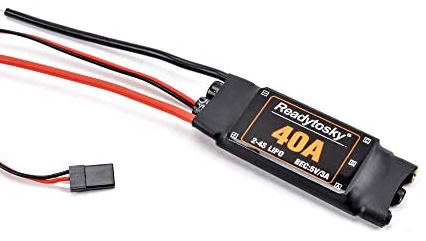
\includegraphics[width=1\linewidth]{esc.png}
        \caption{SpeedyBee BL32 50A 4-in-1 ESC}
        \label{fig:esc50a}
      \end{wrapfigure}

      The SpeedyBee BL32 50A 4-in-1 ESC is a good choice for surveillance drones, and our use case for the following reasons:
      \begin{itemize}
        \item \textbf{\textit{High Current Rating (50A per motor):}} Supports high-thrust motors and larger propellers. Useful for longer flight times, heavy payloads (cameras, sensors, gimbals), and stable cruising. Provides headroom — motors drawing 20–30A will run cooler and more reliably under a 50A ESC.
        \item \textbf{\textit{BLHeli\_32 Firmware:}} Smoother motor response, more efficient power delivery, and better low-end throttle control, which helps in steady hovering and slow maneuvering — perfect for surveillance.
        \item \textbf{\textit{4-in-1 Design:}} Combines 4 ESCs into one board, and reduces weight and wiring complexity. Makes the stack cleaner, ideal for modular or compact drone frames. Fewer potential failure points (vs. 4 individual ESCs).
        \item \textbf{\textit{Telemetry \& Monitoring:}} Supports ESC telemetry (RPM, current, temperature) via BLHeli\_32. This is important for diagnostics, health monitoring, and autonomous missions — ensuring no motor overheats or fails mid-flight.
        \item \textbf{\textit{Built for 3–6S LiPo:}} Offers flexibility across drone designs. For surveillance, a 4S or 6S setup is common due to higher efficiency and flight duration. This ESC handles both without issue.
        \item \textbf{\textit{Built-in TVS Protection:}} Has \textbf{Transient Voltage Suppression diodes} that protect against voltage spikes — vital for drone safety, especially in critical missions.
      \end{itemize}

      \begin{table}[H]
      \centering
      \caption{ESC Datasheet (SpeedyBee BL32 50A 4-in-1 ESC)}
        \begin{tabular}{|>{\raggedright\arraybackslash}p{6cm}|>{\raggedright\arraybackslash}p{6cm}|}
          \hline
          \textbf{Parameter} & \textbf{Value} \\
          \hline
          Continuous Current (A)	& 50\\
          PWM Frequency Range (KHz) & 16 to 128\\
          Input Power (W)	& 3-6S LiPo \\
          Current Sensor Input	& Support (Scale=490 Offset=0) \\
          Mounting Hole Diameter (mm)	& 30.5 x 30.5mm( {\small 4mm hole diameter}) \\
          Length (mm)	&          45.6\\
          Width (mm)	&      40 \\
          Height (mm)	&        8.8 \\
          Weight (g)	& 19.2g with heat sink\\
          Shipping Weight	& 0.09 kg \\
          Shipping Dimensions	& 12 × 5.8 × 3 cm \\
          \hline
        \end{tabular}
      \end{table}
      \vspace{0.5cm}
      \subsubsection{Propellor: HQProp Thin Electric Prop 9×5 (2CCW) Propeller}

      \begin{wrapfigure}{r}{0.3\textwidth}
        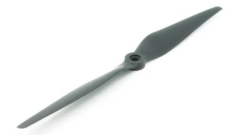
\includegraphics[width=1\linewidth]{prop.png}
        \caption{HQProp Thin Electric Prop 9×5 (2CCW) Propeller}
        \label{fig:prop9x5}
      \end{wrapfigure}

      This propeller is perfect for our use case for the following reasons:

      \begin{itemize}
        \item \textbf{\textit{High Efficiency for Long Endurance Flights:}} It is Thin electric profile = low drag → reduces current draw. Designed for cruise efficiency over brute force thrust, it serves perfect for surveillance missions where hovering and slow, steady forward flight dominate.
        \item \textbf{\textit{Optimized for Mid-Sized Motors (like D2836-7):}} The 9-inch diameter is a good disc area for smooth lift, and 5-inch pitch gives moderate speed per RPM (good forward motion without excess current). These features allows it to pair well with 1000–1200KV motors on 3S LiPo → ideal thrust-to-efficiency balance.
        \item \textbf{\textit{Smooth Throttle Response:}} Thin blades create less turbulence and vibration. This is crucial for gimbal-mounted cameras or FPV systems, reducing jello and image blur.
        \item \textbf{\textit{Expected Performance on 3S + DYS D2836-7:}} 
          \begin{enumerate}
            \item Static Thrust \hfill 850--1000g
            \item Current @ full throttle \hfill 15--18A
            \item Thrust Efficiency \hfill $\approx$ 60--65 g/W
          \end{enumerate}
      \end{itemize}
      \begin{table}[H]
      \centering
      \caption{Propeller Datasheet (HQProp Thin Electric Prop 9×5 (2CCW) Propeller)}
        \begin{tabular}{|>{\raggedright\arraybackslash}p{6cm}|>{\raggedright\arraybackslash}p{6cm}|}
          \hline
          \textbf{Parameter} & \textbf{Value} \\
          \hline
          Material & Carbon Fiber Composite\\
          Rotation Direction	& CCW\\
          Pitch(inch)	& 5\\
          No. of Blades &	2\\
          Hub Diameter (mm)	& 18\\
          Hub Thickness (mm) &	7\\
          Shaft Size (mm) &	9.5/8/6\\
          Adapter Rings (mm) & 6/5/4/3\\
          Weight (g) &	9, (each)\\
          Shipping Weight &	0.035 kg\\
          Shipping Dimensions	& 26 × 6 × 3 cm    \\      
          \hline
        \end{tabular}
      \end{table}

      \vspace{0.5cm}
      
      \subsection{Propulsion Powertrain Efficiency}
      The total powertrain involves all the individual components that draw power from the battery, this includes things like the flight controller and flight computer. Here we are interested only in the propulsion powertrain. The propulsion powertrain typically includes: \[ \text{Battery} \quad \quad \rightarrow \quad \quad  \text{ESC} \quad \quad \rightarrow \quad \quad \text{Motors} \]

      The battery and ESC are suppliers, they supply on demand, and since all 4 motors won't derive the same amount of current (and hence power) at the same point of time-- the real-life parameters will vary in time. Here we assume that all motors demand the same power at all times.\\ \\ To quantify the overall efficiency of the UAV’s propulsion system, we analyze losses in each powertrain component. That is mathematically given by, 
      \[ 
      \boldsymbol{\eta_{total} = \eta_{battery} \times \eta_{esc} \times \eta_{motor}}
      \]
      \textbf{Note:} There are other components in the powertrain which we have not discussed here, and which we have discussed later in this report. Here we are only interested in Propulsion powertrain. \\

      In order to calculate each of these components, we would need to calculate the power input and output at each stage. Since we don't currently have access to each component at the moment to calculate the parameters ourselves, we're going to use the parameters provided by the manufacturers for this calculation. \\ \\
      \textbf{\large Battery Efficiency Derivation:}\\
      Given are the following from datasheets:
      \begin{itemize}
        \item Voltage (V): \hfill 11.1V
        \item Max Discharge Current: \hfill 208.0A (40C)
        \item Max Power Output ($ P_{battery} $): \hfill V x I = 11.1 x 208 = \textbf{2308.8 W}
      \end{itemize}
      This output power from the battery shall be used as input to the ESC. Now, to calculate the efficiency of battery, we can define it as, \[ \eta_{battery} = \frac{P_{out}}{P_{stored}} \] But in-flight, it's more feasible to model this using internal resistance. So, 
      \begin{gather*}
        \text{Power lost in battery} = I^2 \, R_{int} \\
        \eta_{battery} = \frac{VI - I^2 R_{int}}{VI} \,\, = \,\, 1 - \frac{IR_{int}}{V}
    \end{gather*}
    Typically, for our battery, the internal resistance is $ \boldsymbol{R_{int} = 0.015 \Omega} $

    \begin{gather*}
      \text{Power loss} = (208)^2 \times 0.015 = 648.96 \, \text{W} \\
      P_{out} = 11.1 \times 208 = 2308.8 \, \text{W} \\
      P_{stored} = 2308.8 + 648.96 = 2957.76 \, \text{W} \\ \\
      \boldsymbol{\eta_{battery}} = \frac{2308.8}{2957.76} \quad \approx \quad 78.07\, \% \quad = \boldsymbol{0.78}
    \end{gather*}
      \textbf{\large ESC Efficiency Calculations:}\\
      The following data from the datasheets:
      \begin{itemize}
        \item Max Continuous Current:	\hfill50A (per channel)
        \item Voltage Range:\hfill	3–6S LiPo (up to 25.2V)
        \item Estimated Losses:\hfill	~5–10\% (heat dissipation)
      \end{itemize}
      Since this is a 4-in-1 ESC, it shares a single power input from the battery and distributes it internally to all 4 ESC channels. The output power is given by,
      \begin{gather*} 
        P_{out} = P_{in} - P_{loss}\\
        \Rightarrow P_{out} = 2308.8 - \frac{5}{100} \times 2308.8 \\
        \therefore P_{out} \,\, \approx \,\, 2193.36 \, W \\ \\
        \Rightarrow \boldsymbol{P_{in} = 2308.8W} \quad \quad \boldsymbol{P_{out} = 2193.36W} \\ 
        \boldsymbol{\eta_{esc}} = \frac{P_{out}}{P_{in}} = \frac{2193.36}{2308.8} \quad \approx \quad \boldsymbol{0.95}
      \end{gather*}
      The total power output shared by all 4-channels of the ESC is \textbf{2193.36W}. A single channel is capable of supplying, \[ \mathrm{P_{in\_motor}} = \mathrm{P_{out\_ESC}} = \frac{2193.36}{4} = \boldsymbol{548.34 \, \text{W}} \]
      \vspace{0.5in}


      \noindent \textbf{\large Motor Efficiency Derivation:}\\
      The following data is given in the official datasheet:
      \begin{itemize}
        \item KV Rating: \hfill1120 RPM/V
        \item Max Power: \hfill336 W
        \item Max Current: \hfill23.2 A
        \item Voltage Range: \hfill2–4S LiPo (7.4–14.8 V)
        \item Internal Resistance:\hfill 0.070 $\Omega$
        \item Propeller:\hfill 9×5
      \end{itemize}
      The algorithm to derive the motor losses goes as follows: the efficiency is given as,
      \begin{gather*}
        \eta = \frac{\boldsymbol{P_{out}}}{\boldsymbol{P_{in}}}  \\
        \text{Electrical input power:}\quad \boldsymbol{ P_{in} = V \times I} \\
        \text{Mechanical output power:} \quad \boldsymbol{ P_{out} = T \times \omega}
      \end{gather*}
      where \textbf{\textit{V}} is voltage at which thrust is rated, \textbf{\textit{I}} is current drawn at that voltage; \textbf{\textit{T}} is thrust (in newtons), and $ \boldsymbol{\omega} $ is angular velocity given by, 
      \begin{gather*}
        \omega = \frac{2 \pi \times \text{RPM}}{60} \\
        \text{RPM} = 1120 \times 11.1 = 12432.0 \, \,  rpm \\
        \therefore \omega = \frac{2 \pi \times 12432}{60} \approx 1302.45 \, \text{rad/s}
      \end{gather*}
      Now, the mechanical output power is given by \[ \boldsymbol{P_{out} = T \times \omega} \] where T is torque. We can derive it by 
      \begin{gather*}
        \boldsymbol{T = F \times r} \\
        \text{where F} \Rightarrow \text{thrust from propeller (in Newtons)} = 800g \approx 7.8453 \, N \\
        \text{r} \Rightarrow \text{propeller radius (in metres)} = \frac{9in}{2} \approx 4.5in = 0.1143 \, m \\
        \boldsymbol{T = 7.8453 \times 0.1397 = 1.095 \, Nm} \\ \\
        \therefore \boldsymbol{P_{out}} = 1.095 \times 1302.45 \quad \approx \quad \boldsymbol{1426.2 \, W}
      \end{gather*}

      
      %\textbf{Assumptions:}
      %\begin{itemize}
       % \item Battery internal + wiring losses (3\% loss): $\eta_{battery} = 0.97$
        %\item ESC PWM \& Switching Losses: $\eta_{esc} = 0.95$
        %\item Motor (KV rating + loading): $\eta_{motor} = 0.88$
        %\item Propeller thrust efficiency: $ \eta_{prop} = 0.78 $
      %\end{itemize}
  % ======== Aircraft Sizing ========
    \section{Aircraft Sizing}
      \subsection*{Rotor Arm}
      \subsection*{Hub}
      \subsection*{Wheelbase}
      \subsection*{Propeller Clearance}
      \subsection*{Landing Gear}
        
  % ======== Aircraft Performance ====
    \section{Aircraft Performance}
      \subsection{Battery Selection and Endurance}
      \noindent \textbf{Battery: Orange Pro-Range 11.1V 5200mAh (3S)} \\
      \begin{wrapfigure}{r}{0.3\textwidth}
        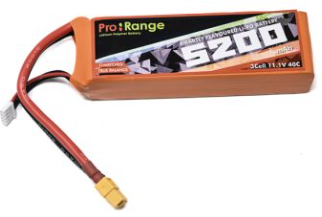
\includegraphics[width=1\linewidth]{battery.png}
        \caption{Orange 11.1V 5200mAh 3S}
        \label{fig:battery3s}
      \end{wrapfigure}
     
      The Orange Pro-Range 11.1V 5200mAh battery is the best for our use case for the following reasons: \\

      The 3S variant provides 11.1V, and has a \textbf{discharge-rate} of 40C. According to the official rated specifications, the maximum continuous discharge current is \textbf{208.0A} (\textit{40C}). It also has a max. burst discharge of \textbf{416.0A} (\textit{80C}). Let us assume that each motor draws 24A current at full-throttle, total current draw would be $ \boldsymbol{24 \times 4 = 96A} $ then \vspace{0.5cm} \[ \text{Theoretical Flight Time (hrs)} = \frac{\text{Capacity (Ah)}}{\text{Current Draw (A)}} = \frac{5.2}{96} \approx 0.0542 hrs = 3.25 mins \] But in real world applications, we dont use 100\% of the battery, we use about 60\%, so that would make the flight time around 5.2mins. 
      \begin{table}[h!]
      \centering
      \caption{Battery and Flight Datasheet Summary (Orange 11.1V 5200mAh 3S)}
        \begin{tabular}{|l|c|}
          \hline
          \textbf{Parameter} & \textbf{Value} \\
          \hline
          Voltage & 11.1V (3S) \\
          \hline
          Capacity & 5.2Ah \\
          \hline
          C-Rating (Continuous) & 35C \\
          \hline
          Theoretical Max Discharge Current & $35 \times 5.2 = \mathbf{182A}$ \\
          \hline
          Stated Max Discharge Current (datasheet) & 156A \\
          \hline
          System Current Draw (4 motors @ 24A) & $4 \times 24 = \mathbf{96A}$ \\
          \hline
              Flight Time @ Full Throttle (96A) & $\frac{5.2}{96} = \mathbf{3.25 \text{ minutes}}$ \\
          \hline
          Flight Time @ Moderate Throttle (60A) & $\frac{5.2}{60} = \mathbf{5.2 \text{ minutes}}$ \\
          \hline
          Energy Capacity & $11.1 \times 5.2 = \mathbf{57.72\,Wh}$ \\
          \hline
        \end{tabular}
      \end{table}
    
      \subsection{Total Power Budget Summary}
        \subsubsection{Propulsion Demand}
        \subsubsection{Avionics Demand}
        \subsubsection{Margins, Safety Factors}
  %========== Material Selection ========
    \section{Material Selection}
      \subsection{Structural Frame, Airframe Components}
    

  %========= Ground Control
    \section{Subystems Selection}
      \subsection{Flight Controller, Sensors, Navigation}
        \subsubsection{Avionics Power Demand}
      \subsection{Communication Systems}

    \section{Autonomous Navigation System}
      \subsection{Hardware Setup}
      \subsection{Software Architechture}

    \section{C.G. Calculation \& Stability Analysis}
      \subsection{Lift, Drag and Stability Considerations}
      \subsection{Center of Gravity Position \& Trim}

  % =========== Computationl Analysis ============
  \chapter{Computationl Analysis}
    \section{CFD / FEM / MATLAB Simulations}
    \section{CAD Model and Performance Validation}
  % =========== Safety, Compliance & Risk Assessment====== 
  \chapter{Safety \& SORA Assessment}
    \section{Risk Analysis and Mitigation Strategies}
      
  % ========= Conclusion & Future Work =====
  \chapter{Methodology for Autonomous Operations}
    \section{Flight Control Algorithm}
    \section{Object Detection \& Counting}
    \section{Autonomous Payload Drop Mechanism (Gripper)}

  \chapter{Innovations and Future Scope}
  \chapter{Bill of Materials}
\end{document}

